
\chapter{Plug-in Environment}

This chapter describes the process of design, implementation and validation of the "Plug-in Environment" feature.


\section{Requirements}

This section described the detailed requirements that regard this feature. In order to identify them we performed additional interviews with the stakeholders. Bellow you can find the requirements described as user stories.


\textbf{TODO Example full usecase}

\textbf{MAYBE say that currently the main problem is that the functions are hardcoded in the workflow engine and cannot be modified without recompiling}

\subsection(What is plug-in?)
custom functionality = Functions + workflows + ....
\textbf{TODO add pictures how plug-ins work}

\section{User stories}
In this section we are formally expressing all the requirements into user stories so that it is more clear and easy to validate.

\begin{itemize}
	\item Add
	
	As a user, I want to easily add custom functionality to U-Sem.
	
	As a user, I want to easily add custom functionality provided by other scientist to U-Sem.
	
	As a user, I don't want to be affected by other users adding new custom functionality.
	
	As a user, I don't want other users to be able to add, delete or modify my custom functionality.
	

	\item Management
	
	As a user, I want to see the list of the custom functionality that is added U-Sem.
	
	As a user, I want to delete custom functionality that has been added to U-Sem.
	
	As a user, I want to be notified about any new versions of the custom functionality provided by other scientists.
	
	As a user, I want to update existing custom functionality with the newest version provided by other scientists.
	
	How to edit workflows(configuration) from plug-in?
	
	\item Usage
	
	As a user, I want to use the added custom functionality in the workflow engine.
	
	As a user, I don't want other users to see what is my custom functionality and use them.

	
\end{itemize}


\section{Background}

OSGI, Eclipse ....

\section{Design}

\subsection{Environment}


\begin{figure}[h!]
  \centering
  	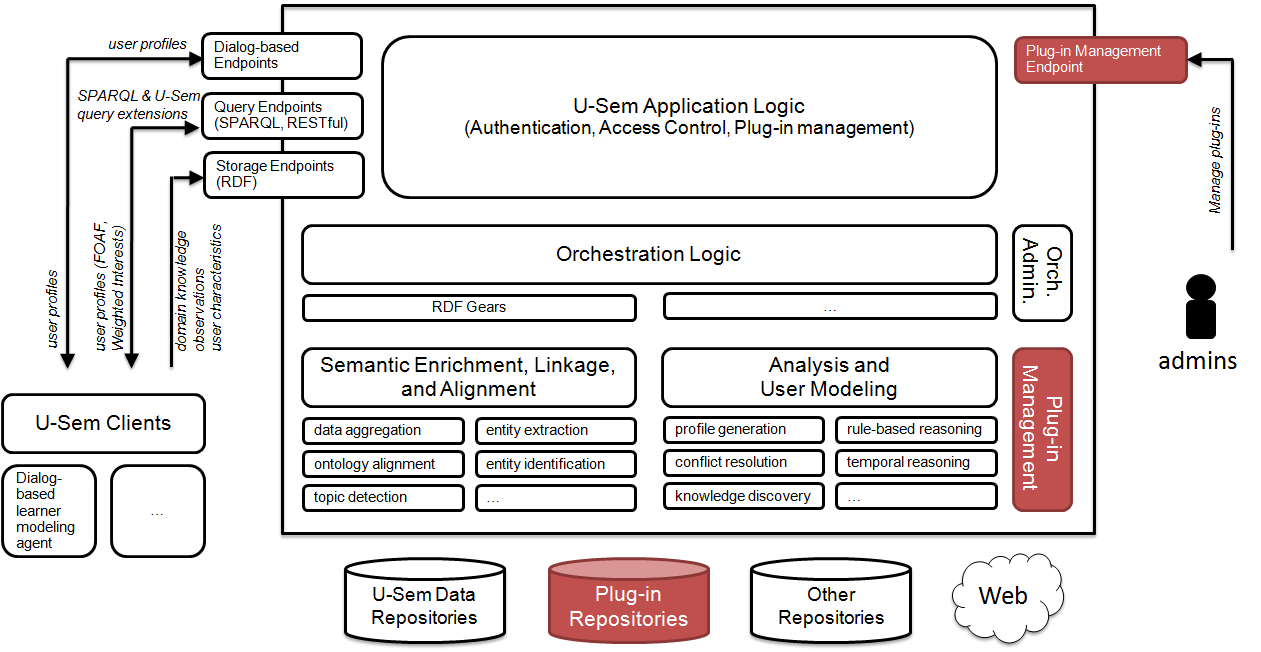
\includegraphics[scale=0.5]{plug-in/Environment.png}
  \caption{The environment in which the system will operate. The components coloured in red build up the Plug-in feature. }
\end{figure}

\subsubsection{Plug-in Management}

This component is responsible to store and manage the access to all plug-ins.

\subsubsection{Plug-in Management endpoint}

This component is responsible to provide endpoint for the administrators to manage the plug-ins. They can install and delete plug-ins.

\subsubsection{Plug-in Repositories}

A Plug-in repository is a storage location from which plug-ins may be retrieved and installed on the system. Scientists build and publish their plug-ins there so that anyone interested in can install and use them.


\subsection{Process modelling}

This section describes how the various component that build this feature interact between each other in order to satisfy the user requirements.

\begin{figure}[h!]
  \centering
  	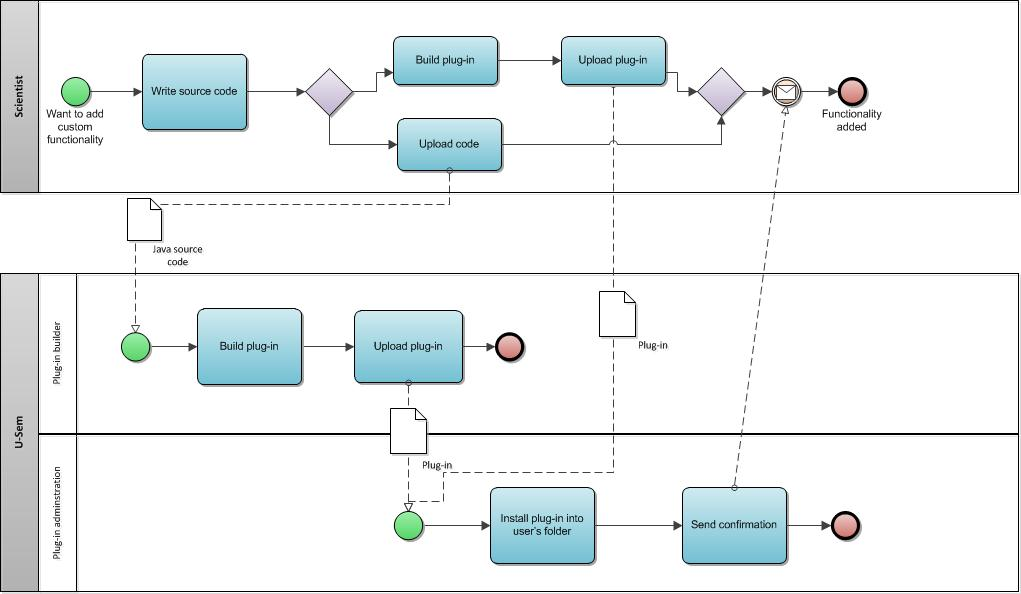
\includegraphics[scale=0.5]{plug-in/AddNewPluginBusinessModel.jpg}
  \caption{Business model describing the process for adding new plug-in to U-Sem}
\end{figure}

\begin{figure}[h!]
  \centering
  	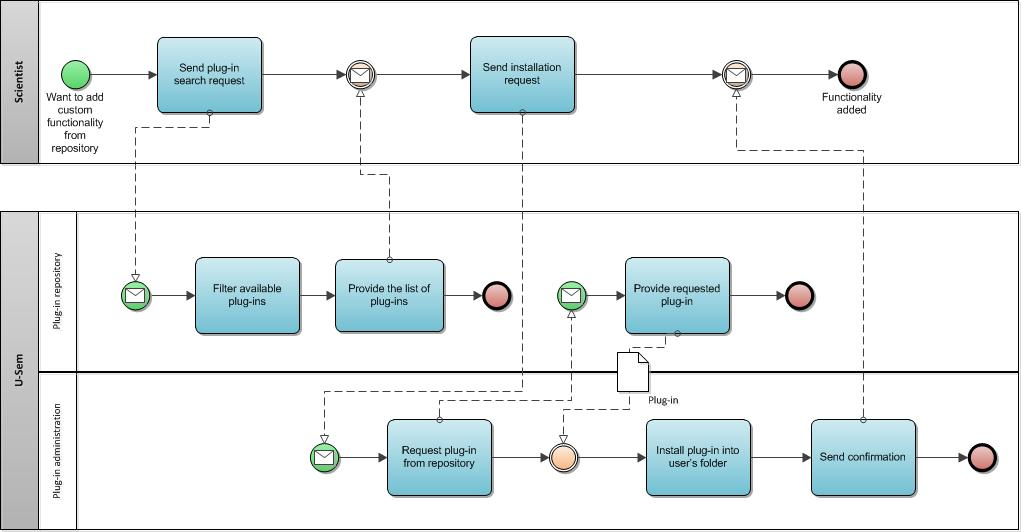
\includegraphics[scale=0.5]{plug-in/AddPlugInFromRepoBusinessModel.jpg}
  \caption{Business model describing the process for adding existing plug-in from repository to U-Sem}
\end{figure}

\subsection{Plugin repository}
\textbf{As new releases of a package are made, other teams can decide whether or not to
immediately adopt the new release. If they decide not to, they simply continue using the
old release. Once they decide that they are ready, they begin to use the new release.
Thus, none of the teams are at the mercy of the others. Changes made to one package
do not need to have an immediate affect on other teams. Each team can decide for itself
when to adapt its packages to new releases of the packages they use.}

\subsection{Functional viewpoint}

\subsection{Deployment viewpoint}

\section{Implementation}


\section{Validation}

In order to make sure that the implemented feature satisfies the requirements we performed an experiment. We tried to extract outside as a plug-in a functionallity that is currently hardcoded into the workflow engine outside


\begin{thebibliography}{99}

\bibitem{Karlsson}
Karlsson, J., Ryan, K. (1997). A Cost-Value Approach for Prioritizing Requirements, IEEE Software September/October 1997, 67-74.


\end{thebibliography}